\documentclass{standalone}
\newcommand{\RR}{{\mathbb{R}}}
\usepackage{tikz}
\usepackage{amsmath}
\begin{document}
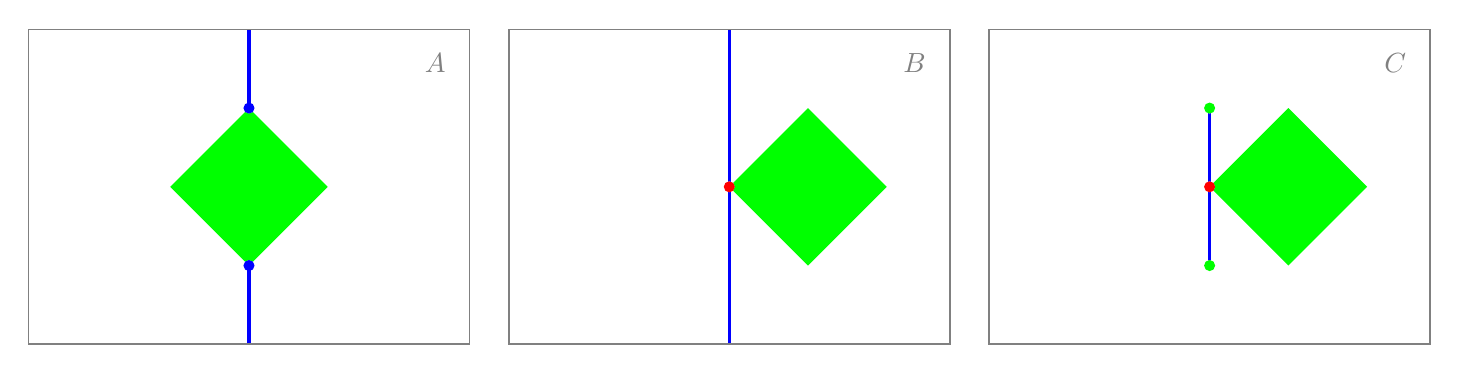
\begin{tikzpicture}
		\draw[gray, line width=0.6pt] (-2.8,-2) rectangle (2.8,2) 
		node[anchor=north east, shift={(-5pt,-5pt)}]{$A$};
		\begin{scope}[even odd rule]
			\clip (-2.8,-2) rectangle (2.8, 2) (0,1) circle(2pt) 
			(0,-1) circle(2pt);
			\fill[green] (0,-1) -- (1,0) -- (0,1) -- (-1,0) -- cycle;
		\end{scope}	
		\draw[blue, line width=1.2pt, shorten <= 0.3pt] 
		(0,-2) -- (0,-1);
		\fill[blue] (0,-1) circle(2pt);
		\draw[blue, line width=1.2pt, shorten <= 0.3pt] 
		(0,2) -- (0,1);
		\fill[blue] (0,1) circle(2pt);
		\begin{scope}[shift={(6.1,0)}]
			\draw[gray, line width=0.6pt] (-2.8,-2) rectangle (2.8,2)
			node[anchor=north east, shift={(-5pt,-5pt)}]{$B$};	
			\begin{scope}[even odd rule]
			\clip (-2.8,-2) rectangle (2.8, 2) (0,0) circle(2pt);
			\fill[green] (1,-1) -- (2,0) -- (1,1) -- (0,0) -- cycle;
			\draw[blue, line width=1.2pt, shorten <= 0.3pt]%, shorten >= 1pt] 
				(0,-2) -- (0,0);
			\draw[blue, line width=1.2pt, shorten <= 0.3pt]%, shorten >= 1pt] 
				(0,2) -- (0,0);
			\end{scope}
			\fill[red] (0,0) circle(2pt);	
		\end{scope}
		\begin{scope}[shift={(12.2,0)}]
			\draw[gray, line width=0.6pt] (-2.8,-2) rectangle (2.8,2) 
			node[anchor=north east, shift={(-5pt,-5pt)}]{$C$};	
			\begin{scope}[even odd rule]
				\clip (-2.8,-2) rectangle (2.8, 2) (0,1) circle(2pt) 
				(0,-1) circle(2pt) (0,0) circle(2pt);
			\fill[green] (1,-1) -- (2,0) -- (1,1) -- (0,0) -- cycle;
			\draw[blue, line width=1.2pt] (0,-1) -- (0,1);
			\end{scope}
			\fill[green] (0,-1) circle(2pt);	
			\fill[green] (0,1) circle(2pt);	
			\fill[red] (0,0) circle(2pt);	
		\end{scope}
	\end{tikzpicture}
\end{document}